\subsection{Comportamiento Esperado de PageRank}
\label{subsec:exp1}
\begin{LaTeXdescription}
    \item[Objetivo] Ejemplificar el comportamiendo esperado de PageRank.
        Proponemos, a su vez, que el orden obtenido por PageRank ser\'a el mismo
        para cualquier factor de navegaci\'on $\alpha$\footnote{Lo llamamos
        ''factor de navegaci\'on'' al par\'ametro $\alpha$ ya que el mismo
        determina el peso/importancia del grafo/matriz de navegaci\'on $S$
        (definida en la ecuaci\'on \ref{eq:S}, p\'agina \pageref{eq:S}). Se
        puede observar en la definici\'on de $M$ en la p\'agina
        \pageref{eq:M_def} que justamente $\alpha$ define en que porporci\'on
        estar\'an inclu\'idos en $S$ y la matriz de teletransportaic\'on
        uniforme. Llamamos entonces a $\alpha$ factor de navegaci\'on, ya
        que de alguna manera nos indica directamente sin tener que pensar en
        $(1-\alpha)$ en que proporci\'on participa $S$ en $M$, y decimos que
        $S$ es una matriz de navegaci\'on ya que es la matriz que contiene
        los datos de la matriz de conectividad con el inconveniente de los
        dangling nodes resuelto.}, aunque las probabilidades del vector
        resultado (asociadas a cada nodo) cambiar\'an seg\'un este
        par\'ametro.\\

    \item[Proposici\'on] No creemos que haga falta aclarar mucho. Ya se
        present\'o y explic\'o m\'etodo a utilizar. Generaremos un grafo de
        entrada lo suficientemente peque\~no que nos permita calcular a mano el
        resultado de PageRank y explicar el porque de su resultado en base al
        conocimiento del m\'etodo.\\

    \item[M\'etodo de Experimentaci\'on] Realizamos la b\'usqueda
        ''site:uba.ar'' en \emph{Google}\cite{google} y tomamos los primeros 10
        resultados.  Generamos una instancia de entrada utilizando las
        herramientas de la c\'atedra y estos 10 resultados. Por \'ultimo, dada
        esta instancia de prueba, calculamos el \emph{ranking} con el m\'etodo
        PageRank para varios distintos factores de navegaci\'on $\alpha$.\\

    \item[Resultados, an\'alisis y discusi\'on]
\end{LaTeXdescription}

\par En la figura \ref{fig:uba.ar_graph} podemos observar el grafo de
conectividad resultante de los 10 resultados obtenidos por la b\'usqueda
realizada en Google. En el mismo se observan 4 dangling nodes conectados al
grafo: \emph{fvet.uba.ar, ffyb.uba.ar, derecho.uba.ar} y
\emph{videos.agro.uba.ar}, mientras que existen otros dos dangling nodes que no
son alcanzados por ninguno de los nodos del grafo expuesto\footnote{Y por lo
tanto, no los hemos graficado.}: \emph{orga2.exp.dc.uba.ar} y
\emph{iigg.sociales.uba.ar}\footnote{Estos dos sitios que originalmente
aparec\'ian en los primeros 10 resultados de Google al momento de realizar este
experimento, ya no lo hacen m\'as.}.

\begin{figure}[H]
    \centering
    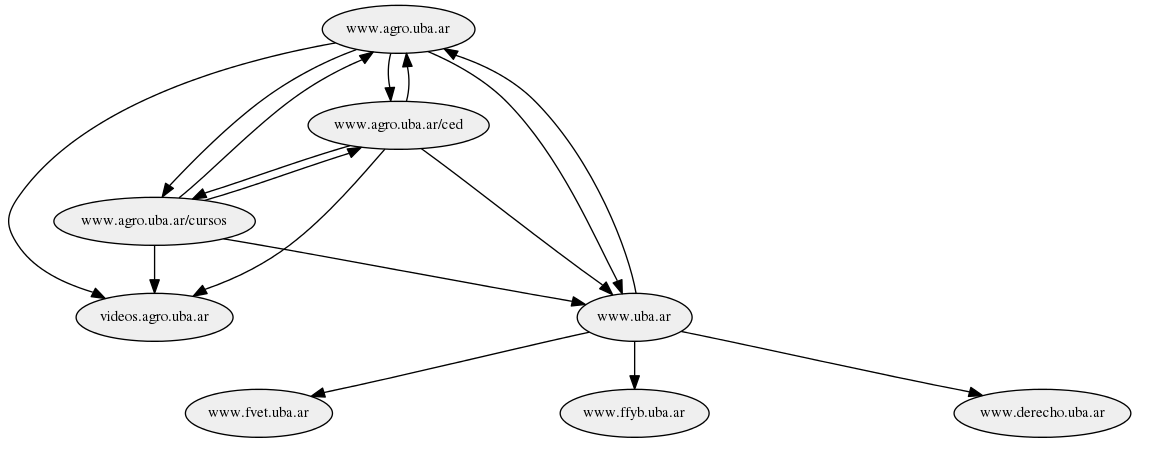
\includegraphics[width=\textwidth]{exp1_conn_graph.png}
    \caption{Grafo de conectividad de la instancia generada con los links
        obtenidos mediante la b\'usqueda en \emph{Google}}
    \label{fig:uba.ar_graph}
\end{figure}

\par As\'i pues, ya podemos comenzar a analizar un poco que es lo que esperamos
encontrar del orden que nos dar\'a PageRank. En primer lugar, los dangling nodes
que est\'an disconexos del grafo consideramos que deber\'ian tener el puntaje
m\'as bajo del grafo, ya que los mismos no tienen backlinks y por lo tanto se
puede pensar que no reciben ning\'un ''voto''. De los restantes dangling nodes,
3 tienen una arista entrante proveniente del mismo nodo, con lo cual esperamos
que estos tengan el mismo puntaje (ya que al recibir una arista cada uno del
mismo nodo, reciben el mismo puntaje de este, pues cada nodo divide por igual su
''poder de voto'' entre todas sus ejes salientes): \emph{fvet.uba.ar,
ffyb.uba.ar, derecho.uba.ar}.

\par De los restantes nodos, podemos observar que tenemos 3 nodos con grado de
entrada 3 (\emph{agro.uba.ar, videos.agro.uba.ar, uba.ar}), y otros 2 nodos con
grado de entrada 2 (\emph{agro.uba.ar/ced, agro.uba.ar/cursos}). Y si observamos
el grado de salida de los nodos (descartando los dangling nodes), tenemos que es
igual a 4. Es decir, todos los nodos dividen su ''poder de voto'' por 4, pero 3
de ellos reciben 3 ''votos'', y los restantes 2 reciben 2 ''votos''. As\'i pues,
para seguir analizando ya debemos observar de donde salen las aristas, ya que de
provenir de un nodo con grado de entrada 3, tendran m\'as peso que de salir de
un nodo de grado de entrada 2.

\smallskip
\begin{description}
    \item[agro.uba.ar] Recibe los votos de: \emph{uba.ar} (grado de entrada
        3), \emph{agro.uba.ar/ced} (grado de entrada 2),
        \emph{agro.uba.ar/cursos} (grado de entrada 2).\smallskip

    \item[videos.agro.uba.ar] Recibe los votos de: \emph{agro.uba.ar} (grado de
        entrada 3), \emph{agro.uba.ar/cursos} y \emph{agro.uba.ar/ced} (ambos
        con grado de entrada 2).\smallskip

    \item[uba.ar] Recibe los votos de: \emph{agro.uba.ar} (grado de entrada 3),
        \emph{agro.uba.ar/cursos} y \emph{agro.uba.ar/ced} (ambos con grado de
        entrada 2).\smallskip

    \item[agro.uba.ar/cursos] Recibe los votos de: \emph{agro.uba.ar} (grado de
        entrada 3), \emph{agro.uba.ar/ced} (grado de entrada 2).\smallskip

    \item[agro.uba.ar/ced] Recibe los votos de: \emph{agro.uba.ar/cursos}(grado
        entrada 2), \emph{agro.uba.ar} (grado de entrada 3).
\end{description}
\medskip

\par Observamos de este resumen que las primeras 3 p\'aginas reciben 3 votos
(uno de grado 3 y dos de grado 2). Las restantes 2 p\'aginas reciben 2 votos
(uno de grado 3 y el restante de grado 2). Con lo cual esperamos encontrar que
estos primeros 3 sitios aparezcan primero en el orden ya que reciben un voto
m\'as, pero ninguno de los 3 deber\'a tener m\'as puntaje que el otro. Seguido
de estos, debemos tener las 2 p\'aginas con 2 votos, nuevamente se repite que
ninguno de estos dos sitios deber\'a tener m\'as votos que el otro.

\par As\'i pues \textit{a priori}, tendr\'iamos un orden obtenido m\'as basado
en los grados de entrada de los nodos, ya que en ning\'un momento observamos que
el ''peso'' de los votos altere el orden que nos dar\'ia \emph{In-Deg}. Sobre
esto desarrollaremos m\'as en el siguiente experimento. Por lo pronto,
observemos el cuadro \ref{tbl:orden_segun_c} para analizar el orden obtenido.

\begin{table}[hb]
    \centering
    \caption{\'Ordenes obtenidos y sus porcentajes para los resultados obtenidos
        de la b\'usqueda ''site:uba.ar'' en \emph{Google}}
    \label{tbl:orden_segun_c}
    \setlength{\tabcolsep}{3pt}
    \begin{tabular}{|l||r||l||r|r|r|r|r|r|r|r|r|}
        \hline
        \multicolumn{2}{|c||}{Caso particular $\alpha = 0$}&
        \multicolumn{10}{c|}{Casos $0 < \alpha < 1$}\\
        \hline
        Orden/P\'agina & 0 & Orden/P\'agina & 0.1&0.2&0.3&0.4&0.5&0.6&0.7&0.8&0.9\\
        \hline\hline
        derecho.uba.ar& 0.1& 
        agro.uba.ar& 0.103548& 0.107198 & 0.110953 & 0.114823 & 0.118812 &
        0.122929 & 0.127182 & 0.131579 & 0.13613\\
        %
        orga2.exp.dc.uba.ar& 0.1&
        uba.ar& 0.103548& 0.107198 & 0.110953 & 0.114823
        & 0.118812 & 0.122929 & 0.127182 & 0.131579 & 0.13613\\
        %
        agro.uba.ar& 0.1&
        videos.agro.uba.ar& 0.103548& 0.107198 & 0.110953 & 0.114823 & 0.118812
        & 0.122929 & 0.127182 & 0.131579 & 0.13613\\
        %
        ffyb.uba.ar& 0.1&
        agro.uba.ar/cursos& 0.101023& 0.102093 & 0.103212 & 0.104384
        & 0.105611 & 0.106895 & 0.10824& 0.109649 & 0.111127\\
        %
        uba.ar& 0.1&
        agro.uba.ar/ced& 0.101023& 0.102093 & 0.103212 & 0.104384
        & 0.105611 & 0.106895 & 0.10824& 0.109649 & 0.111127\\
        %
        fvet.uba.ar& 0.1&
        derecho.uba.ar& 0.0984973& 0.0969883& 0.0954716& 0.0939457&
        0.0924093& 0.0908605& 0.0892978& 0.0877193& 0.0861231\\
        %
        videos.agro.uba.ar& 0.1&
        ffyb.uba.ar& 0.0984973& 0.0969883& 0.0954716& 0.0939457
        & 0.0924093& 0.0908605& 0.0892978& 0.0877193& 0.0861231\\
        %
        iigg.sociales.uba.ar& 0.1&
        fvet.uba.ar& 0.0984973& 0.0969883& 0.0954716& 0.0939457
        & 0.0924093& 0.0908605& 0.0892978& 0.0877193& 0.0861231\\
        %
        agro.uba.ar/cursos& 0.1&
        orga2.exp.dc.uba.ar& 0.0959086& 0.0916284& 0.0871502& 0.0824635& 0.0775579&
        0.0724212& 0.0670411& 0.0614038& 0.0554939\\
        %
        agro.uba.ar/ced& 0.1&
        iigg.sociales.uba.ar& 0.0959086& 0.0916284& 0.0871502& 0.0824635
        & 0.0775579& 0.0724212& 0.0670411& 0.0614038& 0.0554939\\
        %
        \hline\hline
        Probabilidad Total& 1&
        Probabilidad Total& 0.9999991& 1.0000017& 0.9999982& 1.0000011&
        1.0000017& 1.0000009& 1.0000016& 1.0000005& 1.0000011\\
        \hline
    \end{tabular}
\end{table}

\par Lo primero que debemos se\~nalar es que para obtuvimos siempre el mismo
orden (con distintos valores de convergencia/probabilidad de permanencia) para
$0 < \alpha < 1$; y \'unicamente obtuvimos un orden distinto para $\alpha = 0$.

\par En el caso $\alpha = 0$, esto ocurre pues la matriz $M$ pasa a ser una
matriz tal que $m_{ij} = \rfrac{1}{n}$ para todo $i,j$. Recordemos como era la
definici\'on de $M$ de la ecuaci\'on \ref{eq:M_def}:

\begin{align*}
    M &= \alpha S + (1-\alpha) \frac{1}{n}ee^T \quad\quad\quad \alpha\in\real
    \land \alpha\in\left[0,1\right)\\
    %
    \intertext{Luego, para $\alpha = 0$, tenemos que:}
    M &= 0S + \frac{1}{n}ee^T\\
    M & = \frac{1}{n}ee^T
\end{align*}

\par Por lo tanto, para este caso particular, tenemos una matriz que nos
representa un grafo completo y completamente equiprobable. Es decir, volviendo a
la idea del navegante aleatorio de la secci\'on \ref{sec:introduccion}, que no
importa donde se encuentre el navegante, el mismo se ''mover\'a'' a cualquier
p\'agina web del grafo con la misma probabilidad. As\'i pues, tenemos que en
realidad el navegante deber\'ia pasar la misma cantidad de tiempo en todas las
p\'aginas, lo que explica que el orden devuelto para este caso nos d\'e una
probabilidad de $0.1$ para todas las p\'aginas web/nodos. Claramente aqu\'i el
orden en que PageRank devuelve los sitios se debe a una cuesti\'on del orden de
entrada en cual fueron ingresados los sitios, ya que la coordenada 1 del vector
resultante se corresponde con el sitio 1, la coordenada 2 con el sitio 2, etc.
Si todos los nodos tienen la misma probabilidad, el vector nunca es ordenado
seg\'un las probabilidades y lo que estamos observando es seguramente el orden
en el cual fueron ingresados los nodos.

\par Para el resto de los casos, donde el orden obtenido no cambia, debemos
decir que es un resultado con sentido. La elecci\'on del par\'ametro $\alpha$
afecta a los valores de la matriz $M$ (ecuaci\'on \ref{eq:M_def}, p\'agina
\pageref{eq:M_def}), pero no afecta a la conectividad representada por la
matriz. Y esto \'ultimo es lo que mayor peso tiene en el modelo PageRank.
Claramente puede ocurrir, para valores de $\alpha$ \textbf{muy peque\~nos}, que
el orden sea distinto (tendiendo a equiprobable), pero a medida que este
par\'ametro aumente, cada vez ser\'a menor la injerencia de la
teletransportaci\'on y mayor ser\'a la de la conectividad del grafo/instancia
inicial. En este argumento hay un factor clave que no se est\'a teniendo en
cuenta: el tama\~no de la instancia. La injerencia de la teletransportaci\'on
ser\'a cada vez mayor a medida que tengamos instancias m\'as grandes, pues
tendremos cada vez m\'as subgrafos disconexos que ser\'an convertidos a
fuertemente conexos mediante el agregado de los ejes artificiales. No olvidemos
que el concepto de teletransportaci\'on fue introducido artificialmente para
salvar el escollo de la convergencia del c\'alculo del autovector. Es esperable
entonces que a medida que estos ejes artificiales toman menor injerencia
(recordar la definici\'on de $M$) ya sea por un $\alpha$ muy grande y/o un
tama\~no de instancia chico\footnote{Recordemos que las instancias de este tipo
suele crecer en nodos mucho m\'as que en aristas.} m\'as se ''acent\'ue'' el
orden basado en la premisa de PageRank: mayor puntaje a aquellos que tienen la
mejor relaci\'on \emph{cantidad de votos - calidad de votos} (observar que para
$\alpha=0.9$ la diferencia entre los primeros y los segundos aument\'o, respecto
de la diferencia para $\alpha=0.1$, y lo mismo ocurre con los \'ultimos). Aunque
esto ocurre en ambas direcciones, a mayor tama\~no de instancia, seguramente
obtendremos distintos ordenes con $\alpha$ cada vez mayores.

\par Otra observaci\'on que podemos hacer pasa por la evoluci\'on de los
porcentajes para los distintos $\alpha$ en el intervalo $0.1\dots 0.9$.  Vemos
que a medida que aumenta $\alpha$, la mitad del ranking superior comienza
a incrementar su probabilidad en contraparte con la mitad inferior, que se
decrementa.

\par Si bien observamos que todos los nodos que tiene menos probabilidad a mayor
$\alpha$ son dangling nodes, tambi\'en podemos se\~nalar que hay un dangling
node entre los nodos que aumentan su probabilidad: \emph{videos.agro.uba.ar}.
Entonces, no podemos generalizar y decir que este comportamiento ocurre
dependiendo de si un nodo tiene grado de salida 0 o no.

\par Analicemos entonces que significa aumentar $\alpha$. Recordemos la
ecuaci\'on de $M$ presentada en la secci\'on \ref{sec:introduccion}:

\begin{equation*}
    M = \alpha S + (1-\alpha) \frac{1}{n}ee^T \quad\quad\quad \alpha\in\real
    \land \alpha\in\left[0,1\right) \label{eq:M_def}
\end{equation*}

\par Recordemos tambi\'en que $S$ no es otra cosa que la matriz de conectividad
del grafo, habiendo ya resuelto el inconveniente de los dangling nodes. As\'i
pues, vemos que el factor $\alpha$ maneja la proporci\'on en la que $S$ y la
matriz de distribuci\'on uniforme ($(1/n)ee^T$) componen a $M$, siendo una
inversamente proporcional a la otra. Ergo, al aumentar $\alpha$ aumenta el peso
que tiene $S$ (la cual podemos llamar \emph{la matriz de navegaci\'on}, ya que
se basa en el grafo de conectividad m\'as los dangling nodes con capacidad de
teletransportaci\'on) en $M$. Intuitivamente hablando, esto deber\'ia darle
mayor importancia/probabilidad a aquellos nodos que ya se encontraban en la
matriz de conectividad, ya que en esta los ''pesos'' de los ejes salientes
tienen un peso proporcional a $\alpha$ respecto de la capacidad de
teletransportaci\'on que le agrega a $M$ la matriz de distribuci\'on uniforme.

\par Es razonable, entonces, pensar que a mayor $\alpha$ cobre m\'as peso en el
ranking aquellos nodos que dependen de $S$, y en esta matriz tenemos bien
marcado el esquema de ''votos'' de PageRank: los nodos reciben su puntaje de
acuerdo a la cantidad y ''calidad'' de los nodos que los apuntan. En este
contexto, tiene sentido que la mitad superior del ranking aumente su
probabilidad conforme aumenta $\alpha$, ya que son los nodos a los que
inicialmente $S$ les otorga un mayor puntaje (recordar la definici\'on de $S$ en
la p\'agina \pageref{eq:S}).

\par Para finalizar, debemos hacer notar al lector (sino lo ha hecho ya) que la
suma total de las probabilidades para casi todos los casos difiere de $1$. Esto
no es otra cosa que un nuevo ejemplo de los errores n\'umericos de la
aritm\'etica finita, de los cuales ninguna computadora puede escapar (a lo sumo
puede mitigar sus efectos). Claramente, al correr el m\'etodo de la potencia
para obtener el ranking PageRank, el error n\'umerio podr\'ia incluso afectar a
la convergencia real (pues te\'oricamente ya sabemos que deber\'ia converger).
Una de las medidas para mitigar esto es la de trabajar siempre con vectores
normalizados desde el c\'odigo en cada iteraci\'on del m\'etodo, a pesar de
saber que desde la teor\'ia estos ya deber\'ian estarlo\footnote{Medida que no
tomamos, ya que nos dimos cuenta luego de haber corrido los experimentos.}.

\medskip
\par A lo largo de este experimento analizamos un ejemplo peque\~no para
ilustrar el comportamiento del PageRank. El ejemplo en sí mismo quizás no fue
el \'optimo, ya que llegamos a la conclusi\'on de que para la instanci  a de
prueba PageRank no se comportar\'ia diferente que In-Deg (aunque esto no es tan
grave ya que en el siguiente experimento ahondaremos en esto). Sin embargo, fue
un ejemplo bueno que nos permiti\'o exponer como funciona PageRank, cuando se
comporta como \emph{In-Deg} y, quiz\'as lo m\'as importante de este experimento,
unos primeros an\'alisis de como el factor de navegaci\'on $\alpha$ afecta al
orden y las probabilidades del autovector resultante.
